\documentclass[12pt]{article}
\usepackage{graphicx} % Required for inserting images
\usepackage{tikz}
\usetikzlibrary{external}
\tikzexternalize[prefix=tikz/]
\usepackage[utf8]{inputenc}
\usepackage{placeins}
\usepackage{longtable}
\usepackage{setspace}
\usepackage[backend = biber, style= mla]{biblatex}
\usepackage{csquotes}
\setstretch{1.7}
\usepackage{multicol}
\usepackage[version=4]{mhchem}
\addbibresource{refs.bib}
\RequirePackage{newfloat} %% For placing figures in the right place
\usepackage{fancyhdr} %% For custom headers and footers
\usepackage{caption} %% For custom captions
\usepackage[top=1in,bottom=1in,left=0.75in,right=0.75in]{geometry} 
\usepackage{array}
\usepackage[T1]{fontenc}
\usepackage[english]{babel}
\usepackage{graphicx}
\usepackage{appendix}
\usepackage[siunitx, EFvoltages]{circuitikz}
\usepackage{siunitx}
\usepackage{booktabs}
\usepackage{subcaption}
\usepackage{multirow}
\usepackage{float}
\usepackage{physics}
\usepackage{makecell}
\usepackage[makeroom]{cancel}
\usepackage{enumerate}
\usepackage{hyperref}
    \hypersetup{
    colorlinks=true,
    breaklinks=true,
    citecolor=blue,
    linkcolor=black,
    urlcolor=blue,
    }
\numberwithin{equation}{section}
\usepackage[nottoc, notlot, notlof, numbib]{tocbibind}
\usepackage[labelfont=bf]{caption}
\usepackage{amsfonts,amsmath,amssymb}
\usepackage{fancyhdr} %Fancy Title 
\usepackage{setspace}
\usepackage{array}
    \newcolumntype{P}[1]{>{\centering\arraybackslash}p{#1}}
    \newcolumntype{M}[1]{>{\centering\arraybackslash}m{#1}}
\usepackage{multirow}
\usepackage{blindtext}
\usepackage{listings}
\usepackage{pgfplots}
\usepackage[siunitx]{circuitikz} %[symbols]
\usepackage[outline]{contour} % glow around text
\usetikzlibrary{arrows,arrows.meta}
\usetikzlibrary{decorations.markings}
\tikzset{>=latex} % for LaTeX arrow head
\usepackage{xcolor}
\colorlet{Icol}{blue!50!black}
\colorlet{Ccol}{orange!90!black}
\colorlet{Rcol}{green!50!black}
\colorlet{loopcol}{red!90!black!25}
\colorlet{pluscol}{red!60!black}
\colorlet{minuscol}{blue!60!black}
\newcommand\EMF{\mathcal{E}} %\varepsilon}
\contourlength{1.5pt}
\tikzstyle{EMF}=[battery1,l=$\EMF$, invert]
\tikzstyle{internal R}=[R,color=Rcol,Rcol,l=$r$,/tikz/circuitikz/bipoles/length=30pt]
\tikzstyle{loop}=[->,red!90!black!25]
\tikzstyle{loop label}=[loopcol,fill=white,scale=0.8,inner sep=1]
\tikzstyle{thick R}=[R,color=Rcol,thick,Rcol,l=$R$]
\tikzstyle{thick C}=[C,thick,color=Ccol,Ccol,l=$C$]
\tikzstyle{myswitch}=[closing switch,line width=0.3] %-{Latex[length=3]},
\DeclareMathOperator\arctanh{arctanh}
\newcommand{\myvoltmeter}[2] 
{  % #1 = name , #2 = rotation angle
  \begin{scope}[transform shape,rotate=#2]
  \draw[thick] (#1)node(){$\mathbf V$} circle (11pt);
  \draw[rotate=45,-latex] (#1)  +(-17pt,0) --+(17pt,0);
  \end{scope}
}
\ctikzset{bipoles/thickness=1.2}
\newcommand{\midlabelline}[3]{
   \node (midlabel) at ($ (#1)!.5!(#2) $) {#3};
   \draw[latex-] (#1) --  (midlabel);
   \draw[-latex] (midlabel) -- (#2);
}

\renewrobustcmd{\footcite}[1]{
    \footcite{#1}
}


\floatplacement{graph}{H} %% Graphs are placed in the right place


\makeatletter
\renewcommand{\@floatboxreset} {%
        \reset@font
        \normalsize
        \@setminipage
\centering%<<<<<<<<<<<<<<<<<<<
}
\makeatletter

\DeclareFloatingEnvironment{graph}




%% Table of contents options
\renewrobustcmd{\tableofcontents}{
    \pagestyle{empty}
    \section*{Table of Contents}
    \vspace*{0.5cm}
    \hrule
    \vspace*{0.5cm}
    \@starttoc{toc}
    \newpage
    \setcounter{page}{1}
    \pagestyle{fancy}
    \restoregeometry
}

\NeedsTeXFormat{LaTeX2e}
\ProvidesPackage{main}[2023/05/23 baskerville's Package]
%%Package options
%% This loads all the requiered packages for a proper compilation. However
%% future versions may affect the processing of the document. Therefore, it
%% TODO add version dates to all packages
%% TODO add warnings for outdated packages
\RequirePackage{etoolbox} %% Control sequence commands
\RequirePackage{lipsum} %% Lorem ipsum generator
\RequirePackage{ragged2e} %% For justifying text in Math IA's
\RequirePackage{lastpage} %% For retriving the total number of pages in the
%% typsset document
\babelprovide[import,main]{english} %% Main language
\justifying %% This is a must for Math IA's, and is loaded from the ragged2e:
%% https://ctan.org/pkg/ragged2e?lang=en.

\fancyhead[C]{\small\scshape\@title} %% The title of the document is placed
%% in the center of the header. This is completly optional, and can be removed.
\fancyhead[R]{\small\scshape{\thepage/\pageref{LastPage}}} %% The page number
%% along with the total number of pages is placed in the right side of the
%% footer. This isnt required, but is an asthetic choice.
\fancyfoot{\hrule}


\newcommand{\uvec}[1]{\boldsymbol{\hat{\textbf{#1}}}}


\addbibresource{mla.bib}  



\title{IB Math AA HL Internal Assessment}
\date{\vspace{-2cm}}
\begin{document}
\maketitle

{\LARGE{Determining the Alternating Current as a Function of Time in an RLC Circuit to Tune My Digital Audio Converter}}
\section{Introduction}
\noindent Audio sources fall into two major categories: digital audio converters (DACs) and digital audio players (DAPs), the latter being of higher quality and the industry standard. However, because of the extreme cost associated with high-end DAPs, DACs are far more popular. DACs are not inherently worse, but they are designed for mass production - they are not fine-tuned for a specific pair of headphones but are satisfactory for most types of headphones. As an audiophile, I want to create a fine-tuned audio system using available circuitry by altering the RLC circuit used by my current digital audio converter - the Qudelix-5K. This DAC uses 6 circuits that each drive an alternating current at a frequency range associated with the audio. One circuit is for bass, one for treble, and so forth. There are 2 fundamental phenomena associated with circuits: current $I$ and potential difference, or voltage, $V$. Current is defined as $\frac{dQ}{dt}$, or the rate of charge flowing across a given cross-sectional area per unit of time. In circuits, the movement of charge (current) is facilitated by the electromotive force (emf), which provides a potential difference $\varepsilon$ that accelerates charge. 
\FloatBarrier
\subsection{Components}
Capacitors are components of a circuit generally made up of two parallel metal plates, seen in \textbf{Figure \ref{fig:capacitorgeneral}}. As current flows to a capacitor, an equal but opposite charge accumulates on either plate, establishing an electric field that opposes the flow of current. 
\begin{figure}[h!]
    \centering
    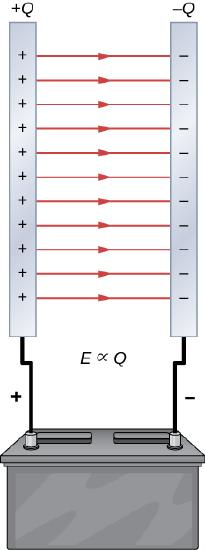
\includegraphics[scale=0.3]{images/capacitor.png}
    \caption{A Standard Parallel-Plate Capacitor}
    \label{fig:capacitorgeneral}
\end{figure}
Capacitance, $C$, is a constant value that quantifies a capacitor's ability to store electric charge. It has units farads ($F$). In an RLC circuit, the charge on the capacitor's plates and its potential difference are both non-constant time functions, denoting $Q$ and $V_C$, respectively. Capacitance is constant as charge and potential differences maintain the same ratio. For a capacitor in an RLC circuit, the charge on either plate $Q =\int_{0}^{t} i(\tau) \, d\tau$, where $\tau$ is the time constant\footfullcite{OpenStax2023Capacitors}. Hence,
\begin{equation}\label{eq:capacitancegeneral}
    C = \frac{Q}{V_C} = \frac{\int_{0}^{t} i(\tau) \, d\tau}{V_C}
\end{equation}
\noindent Inductors, on the other hand, attempt to oppose changes in current by storing energy in a magnetic field $B$. Inductors are quantified by self-inductance, $L$, a measure of how strongly they can oppose changes in $B$ and consequently current. It is given in units Henries ($H$). The potential difference across an inductor $V_L$ is given by:
\begin{equation}\label{eq:inductorvoltage}
    V_L = L\frac{di}{dt}
\end{equation}
\noindent Resistors, even within RLC circuits, are constantly opposite the flow of current. They dissipate a voltage $V_R$, which is given by
\begin{equation}\label{eq:resistancegeneral}
    V_R = iR
\end{equation}
\noindent Where $R$ is the resistance of the resistor, a quantity given in ohms ($\Omega$) that is dependent on temperature. Resistors can be directly implemented into a circuit or can be present in the wire, which will have resistance in non-ideal cases.\\
\FloatBarrier
\begin{figure}[h!]\
    \centering
	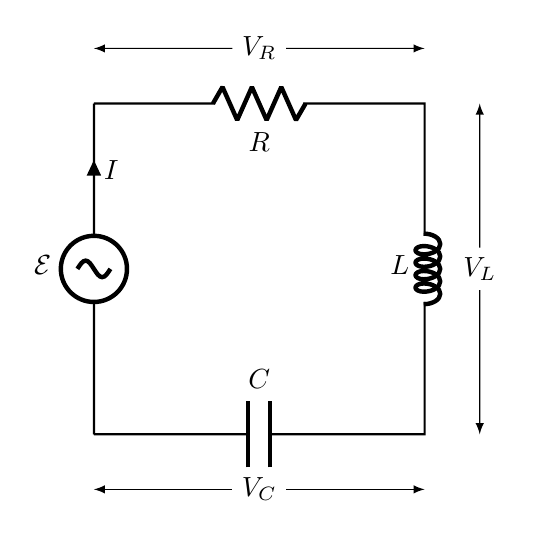
\begin{tikzpicture}[scale=0.7]
		% Circuit
		\draw[line width=0.8]
		 (2,7) to [sinusoidal voltage source, l_=$\mathcal{E}$, i=$I$] (2,1)
		 (2,7) to [resistor, l_=$R$] ++(6,0) to [inductor, l_=$L$] ++(0,-6) to [capacitor, l_=$C$] +(-6,0) ;
		 
		% Voltage Infos
		\midlabelline{2,8}{8,8}{$V_R$}
		\midlabelline{9,7}{9,1}{$V_L$}
		\midlabelline{2,0}{8,0}{$V_C$}
		
		% Grid
%		\draw[help lines] (0,0) grid (10,10)	;
	\end{tikzpicture}
    \caption{RLC Circuit}
    \label{fig:MyModel}
\end{figure}
\FloatBarrier
\noindent In a series RLC circuit, seen in \textbf{Figure \ref{fig:MyModel}}, the voltage across the capacitor will drive a current through the inductor, building up a magnetic field around it. The voltage across the capacitor falls to zero as the current flow uses up the charge. At this point, the energy stored in the magnetic field induces a voltage across the inductor to oppose the current change. This induced voltage causes an opposing current to recharge the capacitor with an opposite polarity, thereby using the magnetic field's energy. When the magnetic field is completely depleted, the current will stop, and the charge will again be stored in the capacitor's plates. This cycle continues, creating an alternating current within the circuit.\footfullcite{RLCBook}. In my DAC model, which will be fine-tuned for the Sennheiser IE 900 earbuds, a series RLC circuit leads to a time-changing current $i(t)$ across a signal capacitor dependent on a dielectric. The dielectric acts as a secondary noise filter at higher current/voltage amplitudes, meaning stable volume in audio. I must find the various quantities for $R,L,C$ in my DAC to determine the current function and tune it for various frequencies. Furthermore, the amplitude of this function, which should be sinusoidal, will correspond to the volume and tunings I have made in my personal equalizer. After confirming what adjustments must be made to the frequencies, I can impose these changes through the dielectric constant to determine different dielectric candidates for each circuit.


\section{Describing the Time-Changing Voltage}
To mathematically define my circuit's current as a function of time, I can make use of Kirchoff's Loop Rule, which states that the sum of the voltages used up by the components of a circuit subtracted from the voltages provided by some electromotive force $\mathcal{E}$ in a closed loop is equal to zero.
\begin{equation}{\label{eq:kirchofflaw}}
    \sum V_{loop} = 0 
\end{equation}

\noindent The frequency circuit used in the Qudelix-5k DAC can be modeled as a traditional RLC circuit, seen in \textbf{Figure \ref{fig:MyModel}}\footfullcite{RLC}. The non-ideal wire has a nonzero resistance, so I depicted it as a resistor in series with the capacitor and inductor, which does not affect my calculations but simplifies the model. Using Kirchoff's Law, I derived an expression for the alternating current as a function of time, where $\mathcal{E}$ is the voltage impressed upon the circuit to compensate for the damping of oscillations over time\footfullcite{RLCBook2}, substituting from (\ref{eq:capacitancegeneral}), (\ref{eq:inductorvoltage}), and (\ref{eq:resistancegeneral}).
\begin{equation}\label{eq:differentialequation1}
    V_L + V_C + V_R = \mathcal{E} \Rightarrow
    L \frac{di}{dt} + \frac{1}{C} \int_{0}^{t} i(\tau) \, d\tau + iR = \mathcal{E}
\end{equation}
\noindent This differential equation can be solved to find the current as a function of time. Before I do so, I must find expressions for the capacitance, self-inductance, and resistance of the wire. 
\section{Computing Unknowns}
\subsection{Capacitance}
I found a recreation of the signal capacitor in the Qudelix in AutoCAD,\footfullcite{CapacitorModel} in \textbf{Figure \ref{fig:fullcapmodel}}.
\begin{figure}[h!]
    \centering
    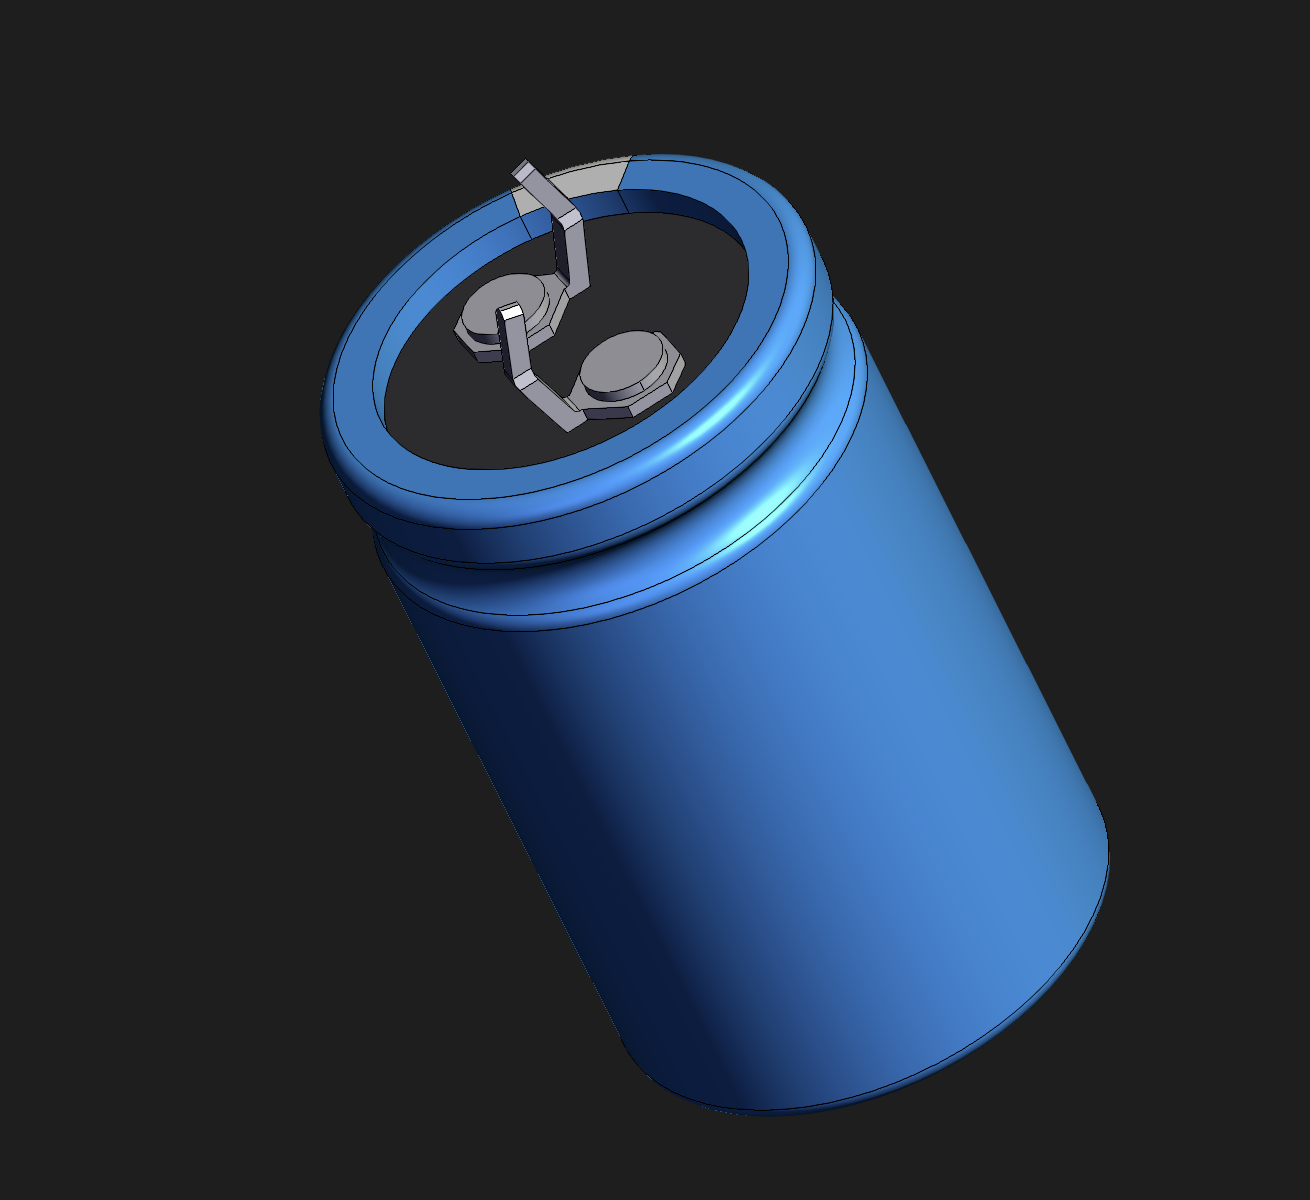
\includegraphics[scale=0.25]{images/capacitormodel.png}
    \caption{Signal Capacitor AutoCAD Model}
    \label{fig:fullcapmodel}
\end{figure}
\noindent As I can see, it is irregularly shaped compared to a normal, parallel plate capacitor. This is a rough recreation, and in actuality, the two protrusions are smooth, with no hard edges, like curved cylinders, and the model is not exactly to scale. In the circuit, two of these capacitors face each other with a maximum separation distance of 6mm, the distance between the bottom circular metal plates of each capacitor. I will use the geometric definition of capacitance:
\begin{equation}\label{eq:capacitorgeometric}
    C = \frac{\kappa \epsilon_0 A}{d}
\end{equation}
\noindent Where $C$ is capacitance, $\kappa$ is the dielectric's relative permittivity, $A$ is the surface area of either metallic surface, $\epsilon_0$ is a constant called the permittivity of free space ($8.85 \times 10^{-12} \, m^{-3} \, kg^{-1} \, s^4 \, A^2$), and $d$ is the average distance between the capacitor plates\footfullcite{DielectricConstants}, which I measured to be 48 cm. I will use (\ref{eq:capacitorgeometric}) to find capacitance as a function of $\kappa$, ranging from close to 0 to over 80000. To find the capacitance of the signal capacitor, I decided to compute the surface area of the metal surfaces, which contain protruding "prongs", using multiple functions for the base plate itself and the protrusions themselves.

\subsubsection{Determining the Area}
The total area is given by 
\begin{equation}\label{eq: areatotal}
    A_1 + 2A_2 = A
\end{equation}
\noindent Where $A_1$ is the visible surface area of the background plates and $A_2$ is the surface area of each prong. Computing $A_1$ is straightforward, I must find the area of the circular background plate, which has radius $R_1$, and subtract from it the area of the 2 screws' base, which has side length $a_s$ and height $h_s$. Then, I must add the surface area of the octagonal screws (excluding the base and the top portion covered by the cylinders) and the cylinders above (also excluding the base) with radius $R_c$ and height $h_c$. 
$$ A_1 = 2 \left[ 2(1+\sqrt{2})a_s^2 - \pi R_c ^2 + 8a_sh_s + 2\pi R_c h_c + \pi R_c^2 \right] + \pi R_1 ^2  = 4 \left[(1+\sqrt{2})a_s^2 + 4a_sh_s + \pi R_c h_c \right] + \pi R_1^2$$
\noindent I measured the unknown quantities by using the back plate as a reference frame in \textbf{Table \ref{tab:measurementsfora1}}:
\begin{table}[h!]
    \centering
    \begin{tabular}{|c|c|} \hline 
       $a_s$  &  0.568 cm\\ \hline 
       $R_C$  &  1.453 cm\\ \hline 
       $h_C$  &  0.236 cm\\ \hline 
       $R_1$  &  9.523 cm \\ \hline 
       $h_s$  &  0.336 cm 
     \\ \hline\end{tabular}
    \caption{Measured Values for Computing $A_1$}
    \label{tab:measurementsfora1}
\end{table}
\FloatBarrier
\noindent Substituting, I found that 
\begin{equation}\label{eq:A_1}
    A_1 = 0.02953814848 \, m^2
\end{equation}
\noindent Now, for the two prongs constituting $A_2$, I decided to approximate a position-height ($x,y$) function for the prong's curve. I used a PlotDigitizer to plot the following points below, and I manually measured the decrease from initial to final height as 0.40 cm. 
\begin{figure}[h!]
    \centering
    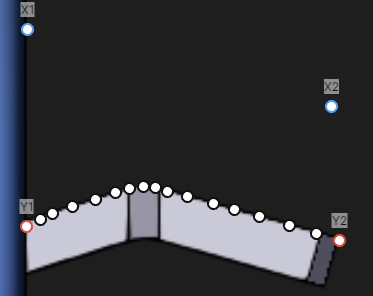
\includegraphics{images/functionforprongs.png}
    \caption{Data Points to Approximate $z_{i} (x)$}
    \label{fig:enter-label}
\end{figure}



\FloatBarrier
\noindent The resulting data points are tabulated in \textbf{Table \ref{table:xydata}}. In conjunction with a function generator, I found the following parabolic best-fit line $z_i (x)$ for these data points:
\begin{equation}
 z_i(x) =-1.15143x^{2}+0.389352x+0.00400807
\end{equation}
Which has roots $x = -0.009998562002, 0.3481450407$. Since the lower side of the prong contains an identical function vertically translated downwards, I needed to find the distance to then create a function for the cylindrical $z_c$. I measured the circumference of the prong, which was roughly 6.28327531 cm, indicating a radius of approximately 1 cm. Hence, I formed the cylinder equation:
\begin{equation}\label{eq:cylinderequation}
    z_c^2 = 0.01^2 + y^2
\end{equation}
From this, I formed the two equations $z_1$ and $z_2$, each representing the top half and bottom half of the prong's surface, respectively.
\begin{equation}
    z_1=\sqrt{0.01^{2}-y^{2}}-1.15143x^{2}+0.389352x+0.00400807
\end{equation}
\begin{equation}
    z_2=-\sqrt{0.01^{2}-y^{2}}-1.15143x^{2}+0.389352x+0.00400807
\end{equation}
Using the two equations, $z_{1,2}$, I graphed the surface modeling the prong.
\begin{figure}[h!]
    \centering
    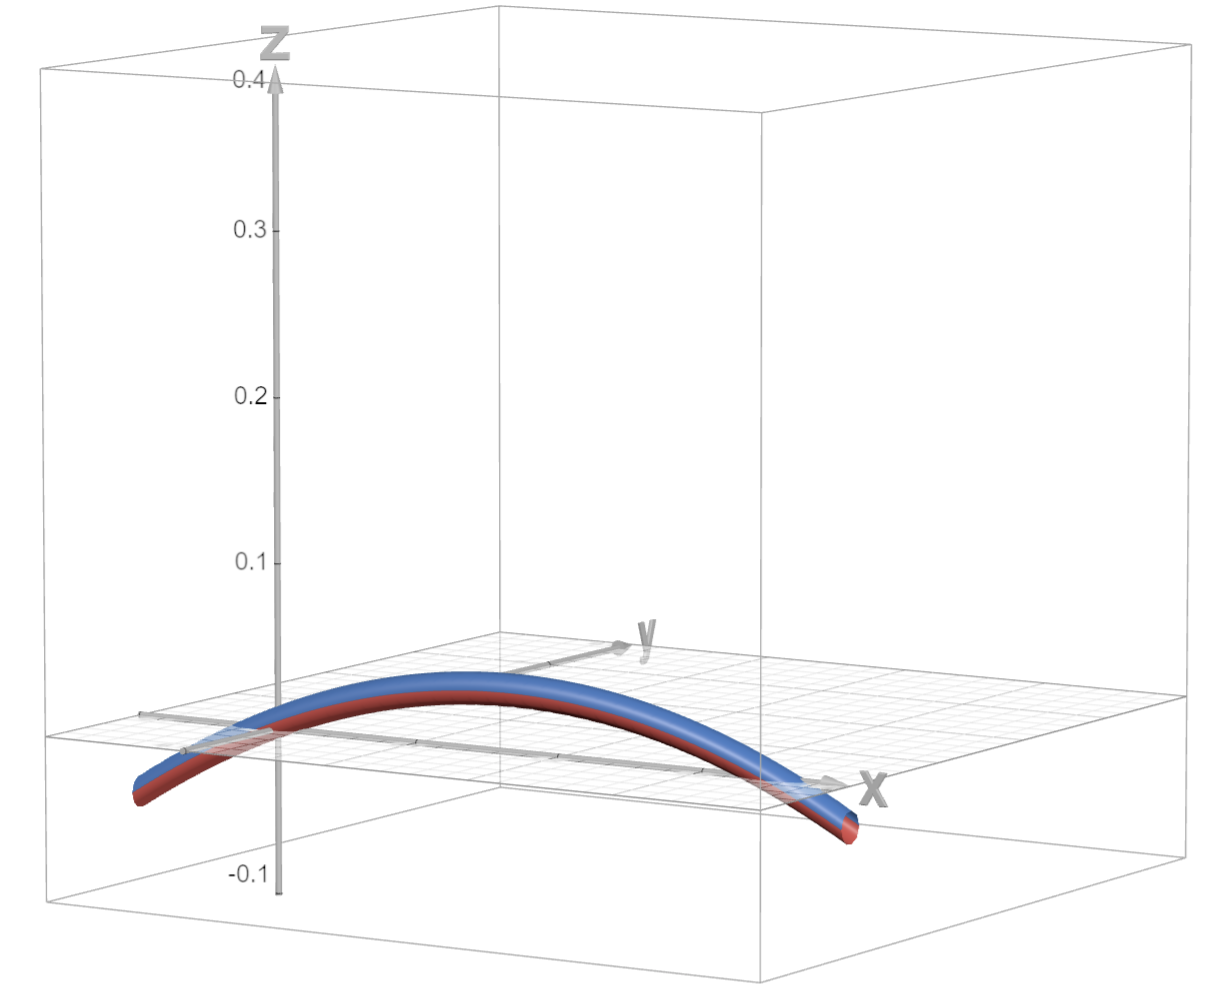
\includegraphics[scale=0.3]{images/prongfunctionfinal.png}
    \caption{$z_1$ and $z_2$}
    \label{fig:fullprongsurface}
\end{figure}
\FloatBarrier
\noindent From the geometry revealed by $z_1$ (blue) and $z_2$ (red), I realized that I could calculate the surface area of this curved cylinder by multiplying the arc length of $z_i$, denoted $S_{z_i}$, with the circumference I measured, the circumference of $z_c$. By the geometry in \textbf{Figure \ref{fig:arclengthfig}}:\FloatBarrier
\begin{figure}
    \centering
    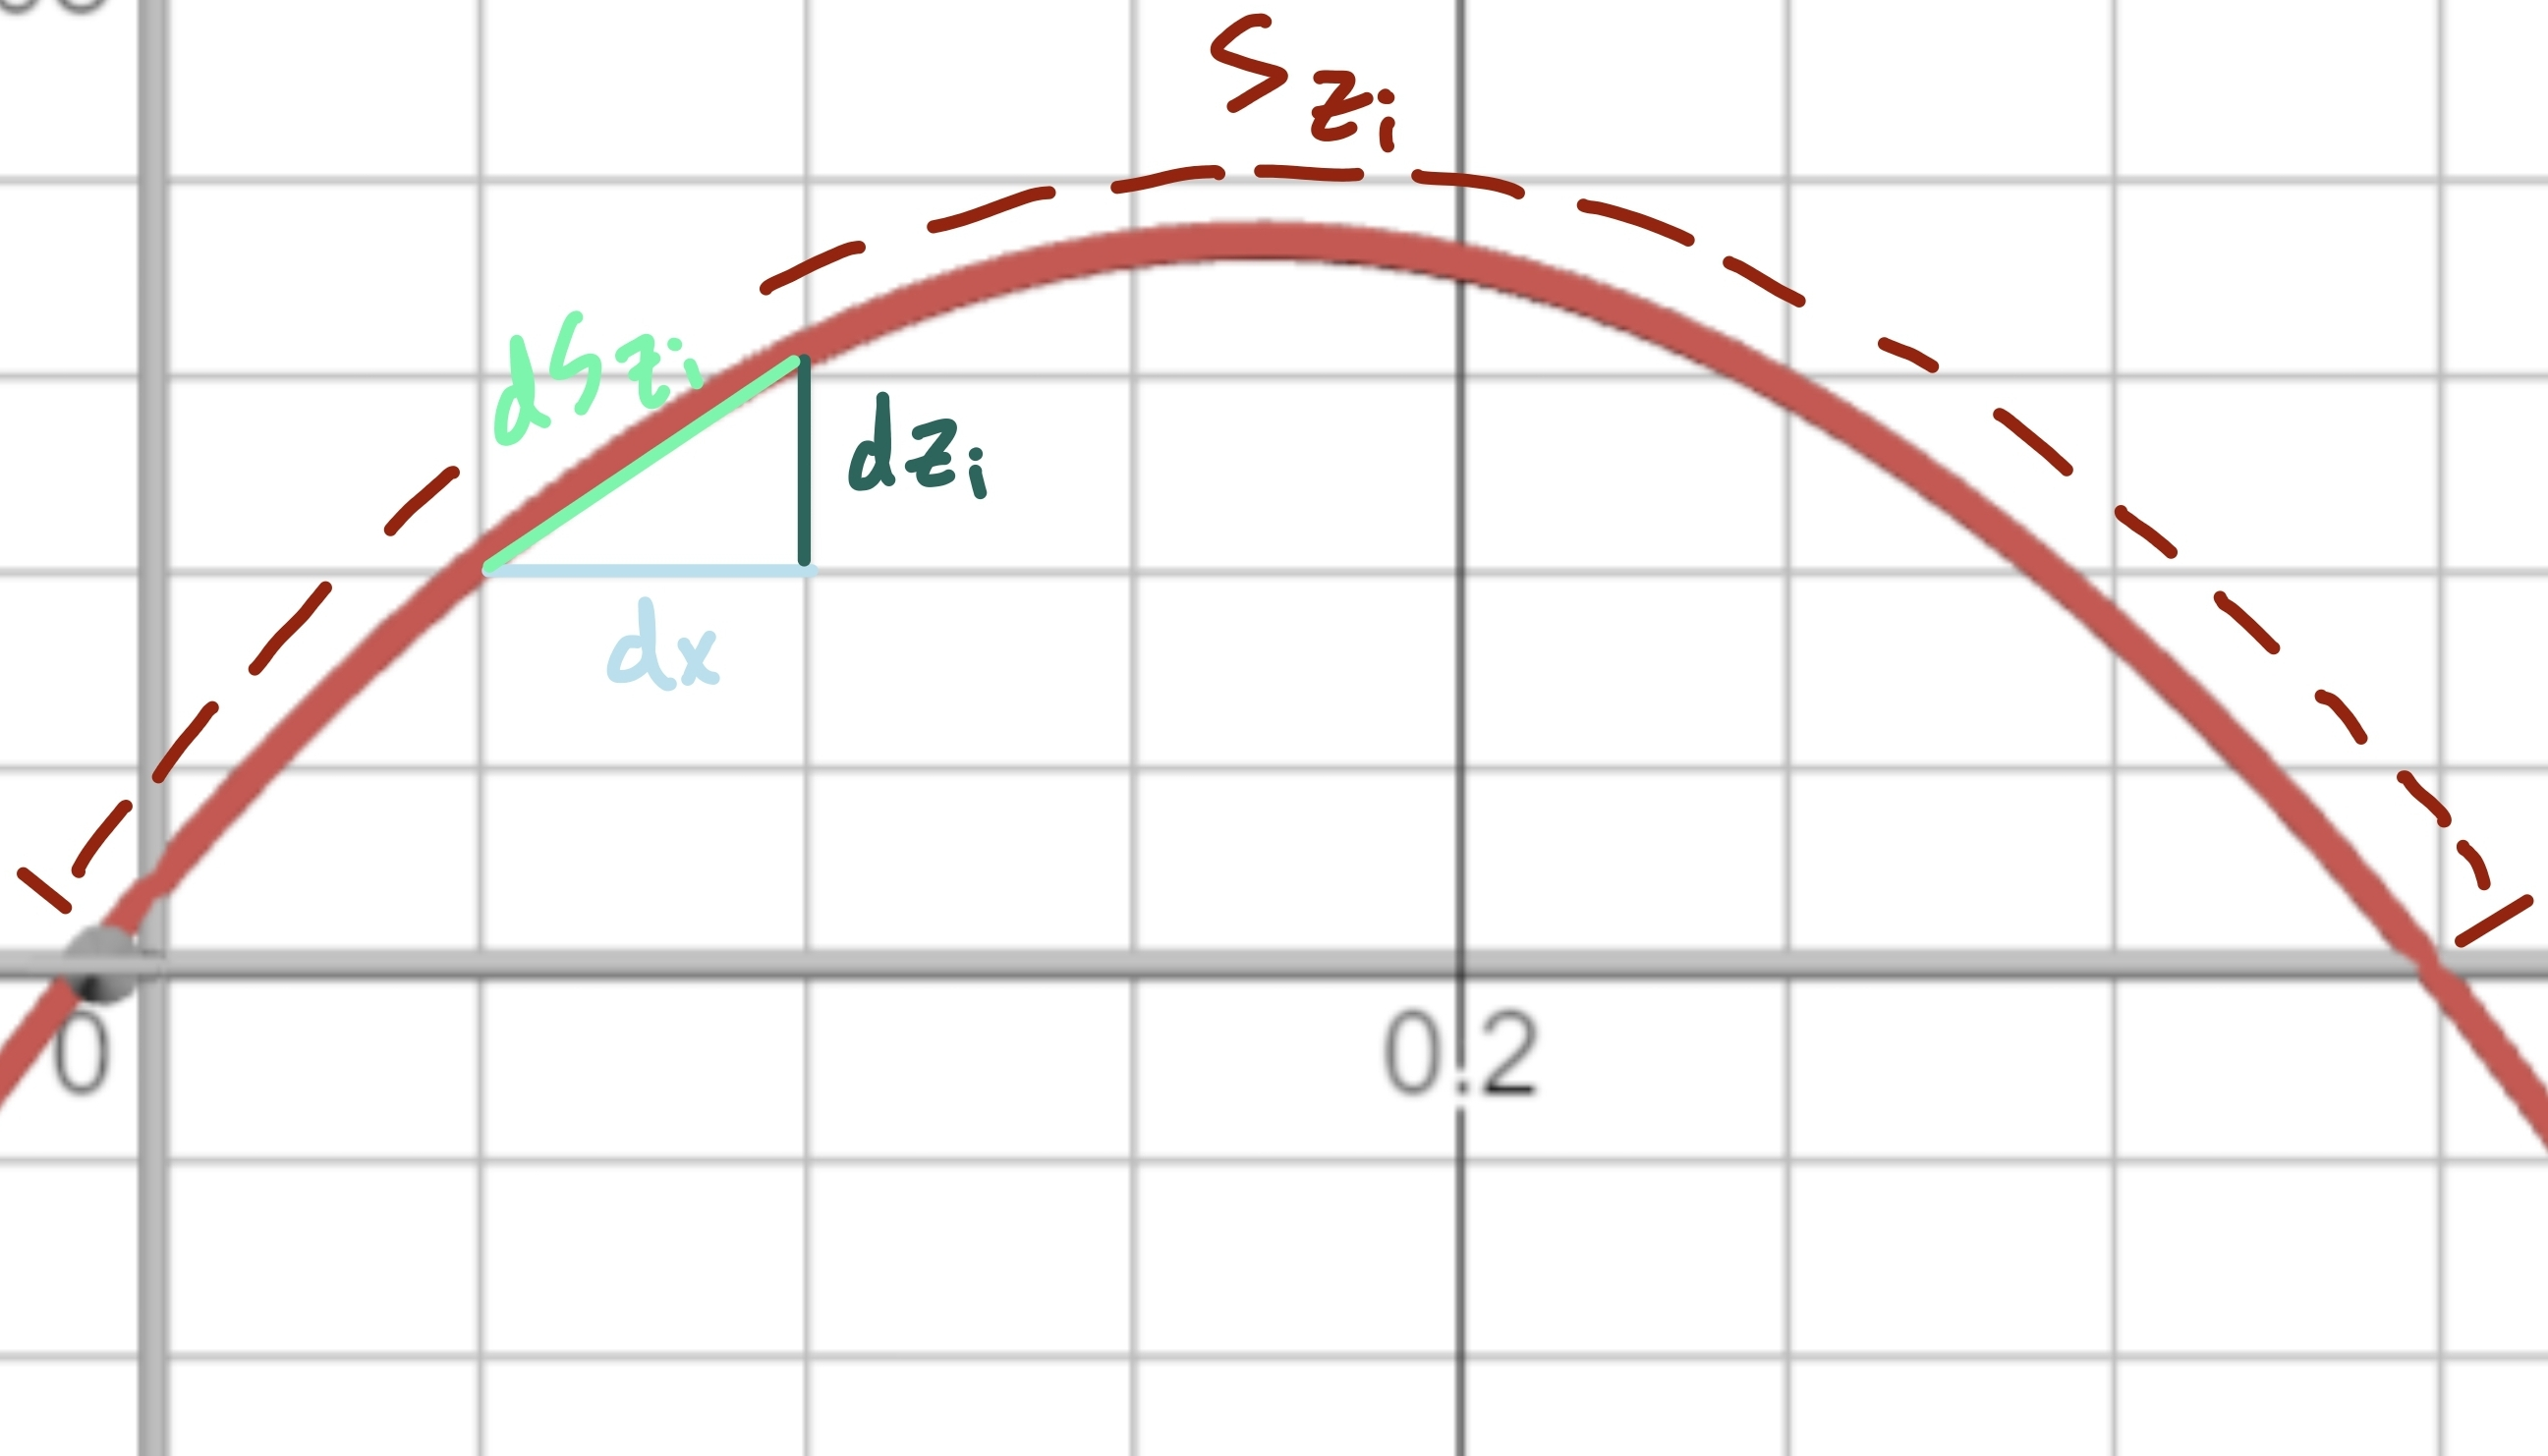
\includegraphics[scale=0.1]{images/arclength2.jpg}
    \caption{Annotated graph of $S_{z_i}$}
    \label{fig:arclengthfig}
\end{figure}
\FloatBarrier
\begin{gather*}
    dS_{z_i} = \sqrt{dx^2 + dz_i^2}\\
    = \sqrt{dx^2 + \left(\frac{dz_i}{dx}dx\right)^2}\\
  \therefore  S_{z_i} = \int_{x_1}^{x_2} \sqrt{1 + \frac{dz_i}{dx}^2} \, dx \\
    \Rightarrow \int_{0}^{0.3481450407} \sqrt{1 + (-1.15143 \cdot 2 \cdot x + 0.389352)^2}  \,  dx
\end{gather*}
\FloatBarrier
\noindent The bounds of the integral are the 0 and the positive root of $z_i(x)$ given the data points' domain. To simplify calculations to solve this integral analytically, I let $b = -1.15143 \cdot 2$ and $c = 0.389352$, ignoring bounds for now and evaluating at the end. The bounds will be  from 0 to $a = 0.3481450407$:
\begin{gather*}
    S_{z_i} = \int \sqrt{1 + (bx+c)^2} \, dx
\end{gather*}
Let $u = bx+c$, hence $dx = \frac{1}{b} du$. Substituting:
\begin{gather*}
   \Rightarrow \frac{1}{b}\int \sqrt{1 + u^2} \, dx
\end{gather*}
Now, let $u = \tan{\epsilon}$, hence 
$$1 + u^2 = \frac{\sin^2{\epsilon} + \cos^2{\epsilon}}{\cos^2{\epsilon}} = \frac{1}{\cos^2{\epsilon}}$$
And $du = \frac{1}{\cos^2{\epsilon}} \, d\epsilon$, so substituting:
\begin{gather*}
    \Rightarrow \frac{1}{b} \int \frac{1}{\cos^3{\epsilon}} \, d\epsilon = \frac{1}{b} \int \sec{\epsilon} \cdot \sec^2{\epsilon} \, d\epsilon
\end{gather*}
Using integration by parts, $u = \sec{\epsilon}$ and $dV = \sec^2{\epsilon} \, d\epsilon$. Hence, $du = \sec{\epsilon} \tan{\epsilon} \, d\epsilon$ and $v = \tan{\epsilon}$. Substituting will yield an indefinite integral that I can then evaluate from the aforementioned bounds for $\epsilon$:
\begin{gather*}
    \Rightarrow \frac{1}{b} \left( \sec{\epsilon} \tan{\epsilon} - \int \sec{\epsilon} \tan^2{\epsilon} \, d\epsilon \right)\\
    = \frac{1}{b} \left( \sec{\epsilon} \tan{\epsilon} - \int \sec{\epsilon} (1-\sec^2{\epsilon}) \, d\epsilon \right)\\
    = \frac{1}{b} \left( \sec{\epsilon} \tan{\epsilon} - \int \sec{\epsilon} \, d\epsilon - \int \sec^3{\epsilon} \,d \epsilon \right) = \frac{1}{b} \int \frac{1}{\cos^3{\epsilon}} \, d\epsilon \\
    \therefore \frac{2}{b} \int \sec^3{\epsilon} \, d\epsilon = \frac{1}{b} \left( \sec{\epsilon} \tan{\epsilon} - \int \sec{\epsilon} \, d\epsilon \right)
\end{gather*}
Simplifying the right-hand side:
\begin{gather*}
    \int \sec{\epsilon} \, d\epsilon = \int \sec{\epsilon} \cdot \frac{\sec{\epsilon} + \tan{\epsilon}}{\sec{\epsilon} + \tan{\epsilon}}  \, d\epsilon \\
    = \int \frac{\sec^2{\epsilon} + \sec{\epsilon}\tan{\epsilon}}{\sec{\epsilon} + \tan{\epsilon}} \, d\epsilon
\end{gather*}
Let $u = \sec{\epsilon} + \tan{\epsilon}$. Hence, $du = \sec^2{\epsilon} + \sec{\epsilon}\tan{\epsilon} \, d\epsilon$. Substituting:
\begin{gather*}
    \Rightarrow \int \frac{du}{u} = \ln{\abs{\sec{\epsilon} + \tan{\epsilon}}}
\end{gather*}
Finally, the original integral for arc length can be expressed as
\begin{equation}\label{eq:finalintegralforarc}
S_{z_i} = \left. \frac{1}{2b} \left( \sec{\epsilon} \tan{\epsilon} - \ln{\abs{\sec{\epsilon} + \tan{\epsilon}}} \right) \right\vert_{\epsilon_1}^{\epsilon_2}
\end{equation}
\noindent Evaluating (\ref{eq:finalintegralforarc}) from the two bounds, which are $\epsilon_1 = \arctan{c}$ and $\epsilon_2 = \arctan{(ab+c)}$, and substituting the numerical values for $a, b, c$ yields (using \textbf{Desmos Scientific Calculator}):
$$S_{z_i} \approx 0.3712934993 \, m $$
\begin{equation}
   \therefore A_2 \approx 2 \pi \cdot 0.01 \cdot 0.3712934993\\
    = 0.0233290586 \, m^2
\end{equation}
\begin{equation}
    \therefore A \approx 0.02953814848 + 2(0.0233290586) = 0.07619626568 \, m^2
\end{equation}
\noindent Now that I have determined the approximate surface area of the capacitor, I can substitute my measured and computed values into (\ref{eq:capacitorgeometric}):
\begin{equation}\label{eq: capacitancevalue}
    C(\kappa) \approx \frac{\kappa (8.85 \times 10^{-12})(0.07619626568)}{0.48} = 1.40486865 \times 10^{-12} \, \kappa F = 1.40486865 \kappa \, \ pF
\end{equation}

\subsection{Determining the Wire's Resistance}
For a wire with constant resistivity $\rho_R$, resistance $R$ is given by

\begin{equation}\label{eq:wireresistance}
    R = \frac{\rho_R L_R}{A_R}  = \frac{\rho_R L_R}{\pi r_R^2}
\end{equation}
\noindent Where $L_R$ is the wire's length (55.3 cm) and $A_R$ is the cross-sectional area of the wire, which has a radius $r_R$ of 1.7 cm. However, the wire I will be using has a nonuniform resistivity, so I rewrite (\ref{eq:wireresistance}) as a differential statement.
\begin{equation}\label{eq:differentialresistivity}
    \frac {dR}{dr} = \frac{d}{dr} \left[ \frac{\rho_R L_R}{\pi r^2} \right] = \frac{\frac{d\rho_R}{dr} L_R \cdot \pi r^2 - 2\pi r \rho_R \cdot L_R}{4\pi^2 r^2} = \frac{L_R}{4\pi} \cdot \frac{\frac{d\rho_R}{dr} r - 2 \rho_R }{r}
\end{equation}
\noindent Where $r$ is the radial distance from the wire's center. I contacted Rheostats, the company from whom I planned to purchase my wiring in my eventual experiment. They scanned the material and gave the following resistivity as a function of ($x,y$), where (0,0) is the center of the wire. The following AutoCAD model was also given. The resistivity function they gave was:

\begin{equation}{\label{eq: resistivityfunc}}
    \rho_R (x,y) = (x^4 +2x^2y^2 +y^4) \left( \frac{-4 \pi^2 \arctanh{\left(\sqrt{1 + \frac{3 (x^8 + 4x^6y^2 + 6x^4y^4 + 4x^2y^6 + y^8)}{5}}\right)}}{\sqrt{5}} \right) , \hspace{10pt} (x,y) \in \mathbb{R}
\end{equation}

\noindent I then parameterized this function using polar coordinates ($x = r\cos(\theta)$, $y = r\sin(\theta)$) to simplify\footnote{Because $\sin^2(\theta) + \cos^2(\theta) = 1$}  and relate the resistivity to (\ref{eq:differentialresistivity}), as the $x^2 + y^2$ terms become $r^2$.
$$ \rho_R (x,y) = \rho_R(r) = r^2 \left( \frac{-4 \pi^2 \arctanh{\left(\sqrt{1 + \frac{3 r^4}{5}}\right)}}{\sqrt{5}} \right) $$

\noindent From this, I found the derivative $\frac{d\rho_R}{dr}$ :
$$
\frac{d\rho_R}{dr} = \frac{8 \pi^2 r}{\sqrt{5} \sqrt{1 + \frac{3 r^4}{5}}} - \frac{8 \pi^2 r \arctanh{\left(\sqrt{1 + \frac{3 r^4}{5}}\right)}}{\sqrt{5}}
$$

\noindent Substituting both into (\ref{eq:differentialresistivity}) and simplifying, I got the following expression for the right side:

\begin{gather*}
\frac{dR}{dr} = \frac{L_R}{4\pi} \cdot \frac{\left( \frac{8 \pi^2 r}{\sqrt{5} \sqrt{1 + \frac{3 r^4}{5}}} - \frac{8 \pi^2 r \arctanh{\left(\sqrt{1 + \frac{3 r^4}{5}}\right)}}{\sqrt{5}} \right) r - 2 \left( r^2 \left( \frac{-4 \pi^2 \arctanh{\left(\sqrt{1 + \frac{3 r^4}{5}}\right)}}{\sqrt{5}} \right) \right)}{r} \\
= \frac{2 \pi r \cdot L_R}{\sqrt{5 + 3r^4}}
\end{gather*}
\noindent Rearranging and integrating both sides, I can solve this differential equation for the total resistance of the wire.
$$  {dR} =  \frac{2\pi r \cdot L_R }{r \sqrt{5+3(r)^4} } dr$$
\begin{equation}\label{eq:resistivityintegral}
    \therefore \int_{0}^{r_R} {dR} =  \int_{0}^{r_R} \frac{2\pi \cdot L_R \, dr}{\sqrt{5+3(r)^4}} 
\end{equation}
The upper bound of the right side integral is the maximum radius of the wire $r_R$, which is 1.7cm. However, integrating this side analytically is beyond the scope of my knowledge, so I decided to approximate the right-side integrand $\nu(r)$ = $\frac{2\pi}{\sqrt{5+3r^4}\cdot L_R}$ as a Maclaurin Series $P(r)$. Because I are integrating over the radius of the wire, which is very close to 0, using a Maclaurin series approximation is suitable and should not impact my results significantly, being much more precise than using Euler's method in this context. In order to find the value of the integral, I decided to expand the integrand using the binomial theorem, letting the common ratio $a = \frac{3}{5}r^4$.

\begin{equation}{\label{eq:maclaurinforrho}}
    \nu (r) = \frac{2\pi \cdot L_R}{\sqrt{5+3r^4}} = \frac{2\pi \cdot L_R}{ \sqrt{5}}\left(1- \frac{3}{5}r^4
 \right)^{-\frac{1}{2}} = \frac{2\pi\cdot L_R}{ \sqrt{5}} \left( 1-a \right)^{-\frac{1}{2}}
\end{equation}
The resulting Maclaurin Series is
$$\nu(r) \approx P(r) = \frac{2\pi\cdot L_R}{\sqrt{5}} \sum_{k=0}^{\infty} \binom{-\frac{1}{2}}{k}\left( \frac{3}{5}r^4 \right)^k = 1 - \frac{1}{2} \left(  \frac{3}{5}r^4 \right) + \frac{3}{8}\left(  \frac{3}{5}r^4 \right)^2 - \frac{5}{16}\left(  \frac{3}{5}r^4 \right)^3 +...$$
$$ \therefore \int_{0}^{r_R} P(r) \, dr =  \frac{2\pi \cdot L_R}{\sqrt{5}}  \int_{0}^{r_R} \sum_{k=0}^{\infty} \binom{-\frac{1}{2}}{k}\left( \frac{3}{5}r^4 \right)^k dr $$
\noindent In order to simplify this further, I checked for the interchangeability of $\int$ and $\sum$ by using the \textbf{Fubini} and \textbf{Tonelli} theorems.\footfullcite{Interchangesumint} Tonelli's theorem states that if a function of $x$, $f_n(x) \geq 0$ for $(n,x) \in \mathbb{R}$, then
\begin{equation}
    \sum \int f_n (x) \,dx = \int \sum f_n(x) \,dx
\end{equation}
On the other hand, Fubini's theorem says that for general $f_n$,
\begin{equation}
   \text{if} \ \sum\int|f_{n}| < \infty \ \text{or} \ \int\sum|f_{n}| < \infty, \ \text{then} \ \sum\int f_{n} = \int\sum f_{n}  
\end{equation}
By Tonelli, the two initial conditions are equivalent. Hence, I first found $\int P(r) \,dr$ by assuming interchangeability and interchanging the integral operator with the sum, as seen in the second condition. This yielded the following expression for the integral, noting that evaluating the integral at $r=0$, or the center of the wire, yielded 0:
\begin{equation}\label{eq: checkwithseries}
\int_{0}^{R} {dR} = R =
\left. 
\frac{2\pi\cdot L_R}{ \sqrt{5}} \sum_{k=0}^{\infty} 
\binom{-\frac{1}{2}}{k} 
\left(\frac{3}{5}\right)^k \frac{(r) ^{4k+1}}{4k+1}  \right \vert_{0}^{r_R}  = 
\frac{2\pi\cdot L_R}{ \sqrt{5}} \sum_{k=0}^{\infty} 
\binom{-\frac{1}{2}}{k} 
\left(\frac{3}{5}\right)^k \frac{(r_R) ^{4k+1}}{4k+1}  \end{equation}
Next, I checked to see if this series absolutely converges. If it does, the sum and integral can be interchanged, and I have already found an expression for the integral. I cannot check convergence with a standard limit or ratio test because my approach yielded an alternating infinite series for which I could not find the general coefficients. This also did not allow me to determine the remainder. Instead, I decided to find the first few partial sums $S_n$. Because $r_R$ is smaller than 1, and consequently $a_n << 1$, that sequence of partial sums should converge very quickly. Then, I will require the next term's contribution to be less than $1\%$ of a given partial sum to determine which one I will use to approximate $R$, as they each represent values for the right side of (\ref{eq: checkwithseries}). The sums were computed with a calculator and are presented in \textbf{Table \ref{tab:partialsums}}:
\begin{table}[h!]
  \begin{center}
  \begin{tabular}{|  c  |c  |c   |c|} \hline    $S_n$ & $\frac{2\pi \cdot L_R}{ \sqrt{5}} \sum_{i=0}^{n} \binom{-\frac{1}{2}}{i} 
\left(\frac{3}{5}\right)^i \frac{(r_R) ^{4i+1}}{4i+1} $ & $a_{n+1}$ & \% \\ \hline   
    $S_0$ & 0.026416113314605548 & $  -1.3237801200895025 \times 10 
^{-10} $ & $  5.01126 \times 10 
^{-7} \, \% $ \\ \hline   
    $S_1$ & 0.026416113182227537 & $ 2.7640859852498835 \times 10^{-18} $ &  $ 1.0463636213936005 \times 10^{-14} \%$ \\ \hline   
    $S_2$ & 0.02641611318222754 & $ -7.991280885255771 \times 10^{-26}$& $ 3.02515393923744 \times 10^{-22} \% $ \\ \hline   
    $S_3$ & 0.02641611318222754 &$ 2.6795743740171055 \times 10^{-33}$ & $ 1.0143711739620698 \times 10^{-29} \%$ \\ \hline 
\end{tabular} 
\end{center}
    \caption{Partial Sums for $R$}
    \label{tab:partialsums}
\end{table}

\noindent The remainder values after $n=3$ were so small that I could not determine them on any given calculator, resulting in the values above. Clearly, the series converges extremely quickly and I can conclude that (\ref{eq: checkwithseries}) converges absolutely. So, I verified that the second condition of Fubini's theorem is fulfilled, hence allowing for the interchanging of the integral and summation in Tonelli's theorem and proving that (\ref{eq: checkwithseries}) is a valid expression for the resistance. To compute $R$, the first term itself sufficed given my requirement with a negligeble remainder, making $S_0$ a very precise approximation of the right side integral in (\ref{eq:differentialresistivity}). I can now solve (\ref{eq:differentialresistivity}) by substituting $S_0$ for the right side:
\begin{gather*}
    \int_{0}^{r_R}{dR} \approx S_0 = 0.026416113314605548\\
    \therefore R = 0.026416113314605548 \, \Omega = Z_R
\end{gather*}
Finally, using Ohm's law, I can find the voltage consumed by the wire as $V_{R}=iZ_R$, or
\begin{equation}\label{eq:wirevoltage}
    iR = \frac{dQ}{dt} \cdot 0.026416113314605548
\end{equation}

\FloatBarrier
\subsection{Determining Self-Inductance}
The solenoid in the Qudelix is modeled in \textbf{Figure \ref{fig:Solenoid3d}}

\begin{figure}[h!]
    \centering
    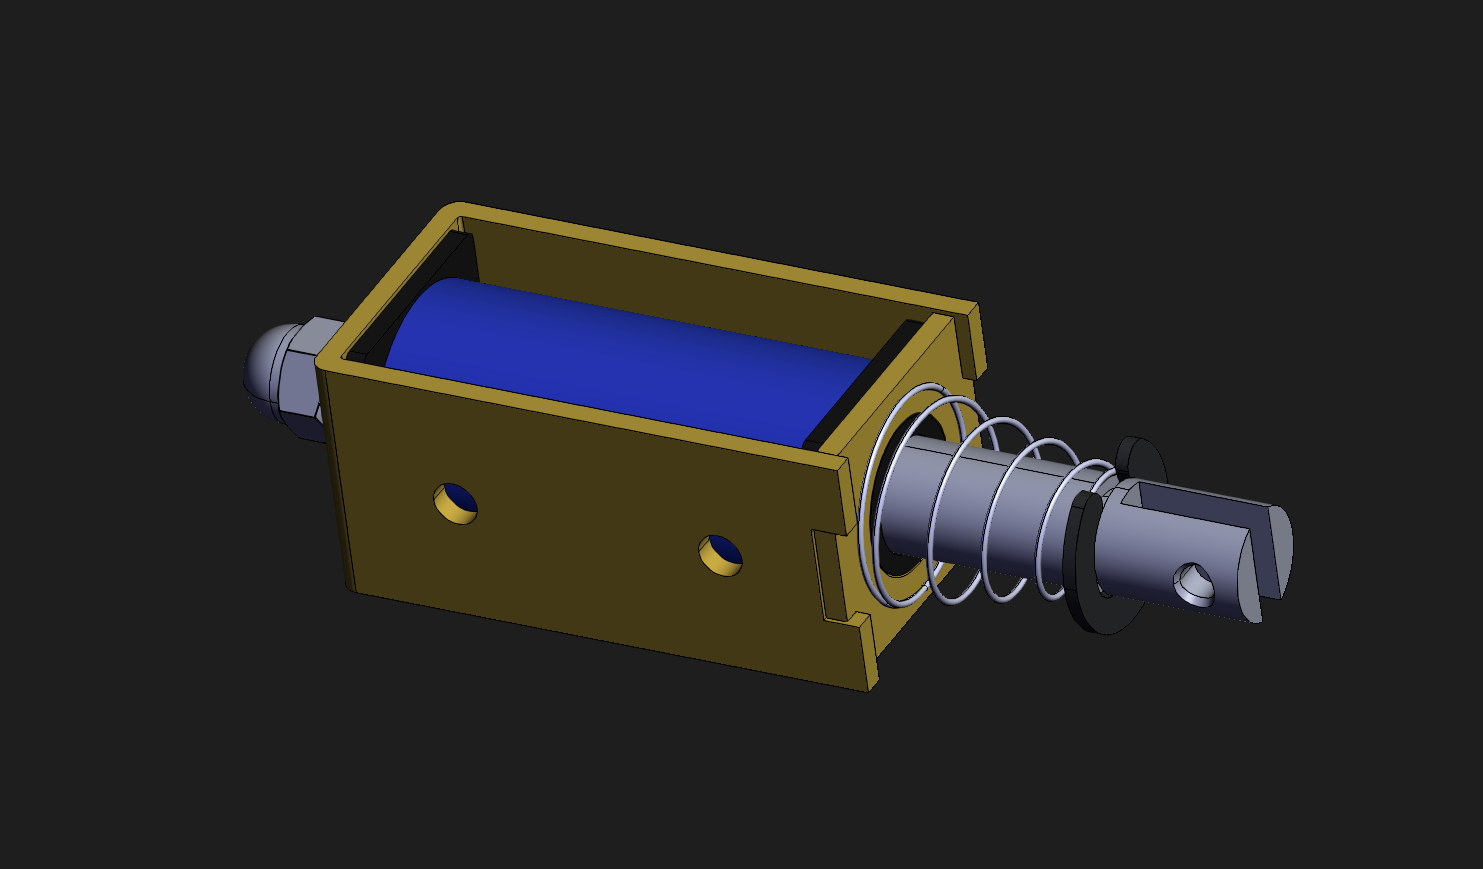
\includegraphics[scale=0.25]{images/solenoid3dd.png}
    \caption{Solenoid 3/4 View}
    \label{fig:Solenoid3d}
\end{figure}

\noindent The self-inductance of a solenoid is given by (\ref{eq:Selfinductancesolenoid}):

\begin{equation}\label{eq:Selfinductancesolenoid}
    L = \frac{\mu_0 N^2 A}{\ell} 
\end{equation}

\noindent Where $\mu_0$ is a constant called the permeability of free space ($4\pi \times 10^{-7} H/m$), $N$ is the total number of turns in the solenoid, $A$ is its cross-sectional area, and $\ell$ is its length. In the \textbf{Figure \ref{fig:Solenoid3d}}, the coiled metal forms the solenoid. Within the enclosed box, the metal continues to coil, with a constant cross-sectional area. In front of the box, however, the cross-sectional area enclosed by each consecutive loop is visibly increasing. By finding a function for $A(x)$ with increasing radius based on position, I can determine a piecewise function for the cross-sectional area and solve for the total self-inductance. Let us first write (\ref{eq:Selfinductancesolenoid}) as a differential statement because the cross-sectional area varies. For a solenoid whose cross-sectional area \( A(x) \) varies with position along its length, I consider a small segment \( dx \) at a position \( x \) along the length of the solenoid. Assuming the turns are uniformly distributed along the length of the solenoid so that the ratio $\frac{dN}{dx} = \frac{N}{\ell}$, the number of turns in this small segment is \({dN} = (N/l)\,dx \). On this tiny segment $dN$, for which the varying area function is approximately constant, a tiny amount of the inductance $dL$ is contributed.
\begin{equation}
    dL = \mu_0 \frac{(dN)^2 A(x)}{dx} = \mu_0 \frac{N^2}{\ell^2} A(x) \,dx
\end{equation}
To find the total inductance of the solenoid, I integrate this expression over the length of the solenoid, to find the contribution of each $dN$ to $L$ while accounting for the varying area:
\begin{equation}\label{eq:Inductanceeq}
    L = \int_{0}^{\ell} \mu_0 \frac{N^2}{\ell^2} A(x) \, dx
\end{equation}

\noindent I then annotated the solenoid model from a side-view in \textbf{Figure \ref{fig:solenoidsideview}}.
\begin{figure}[h!]
    \centering
    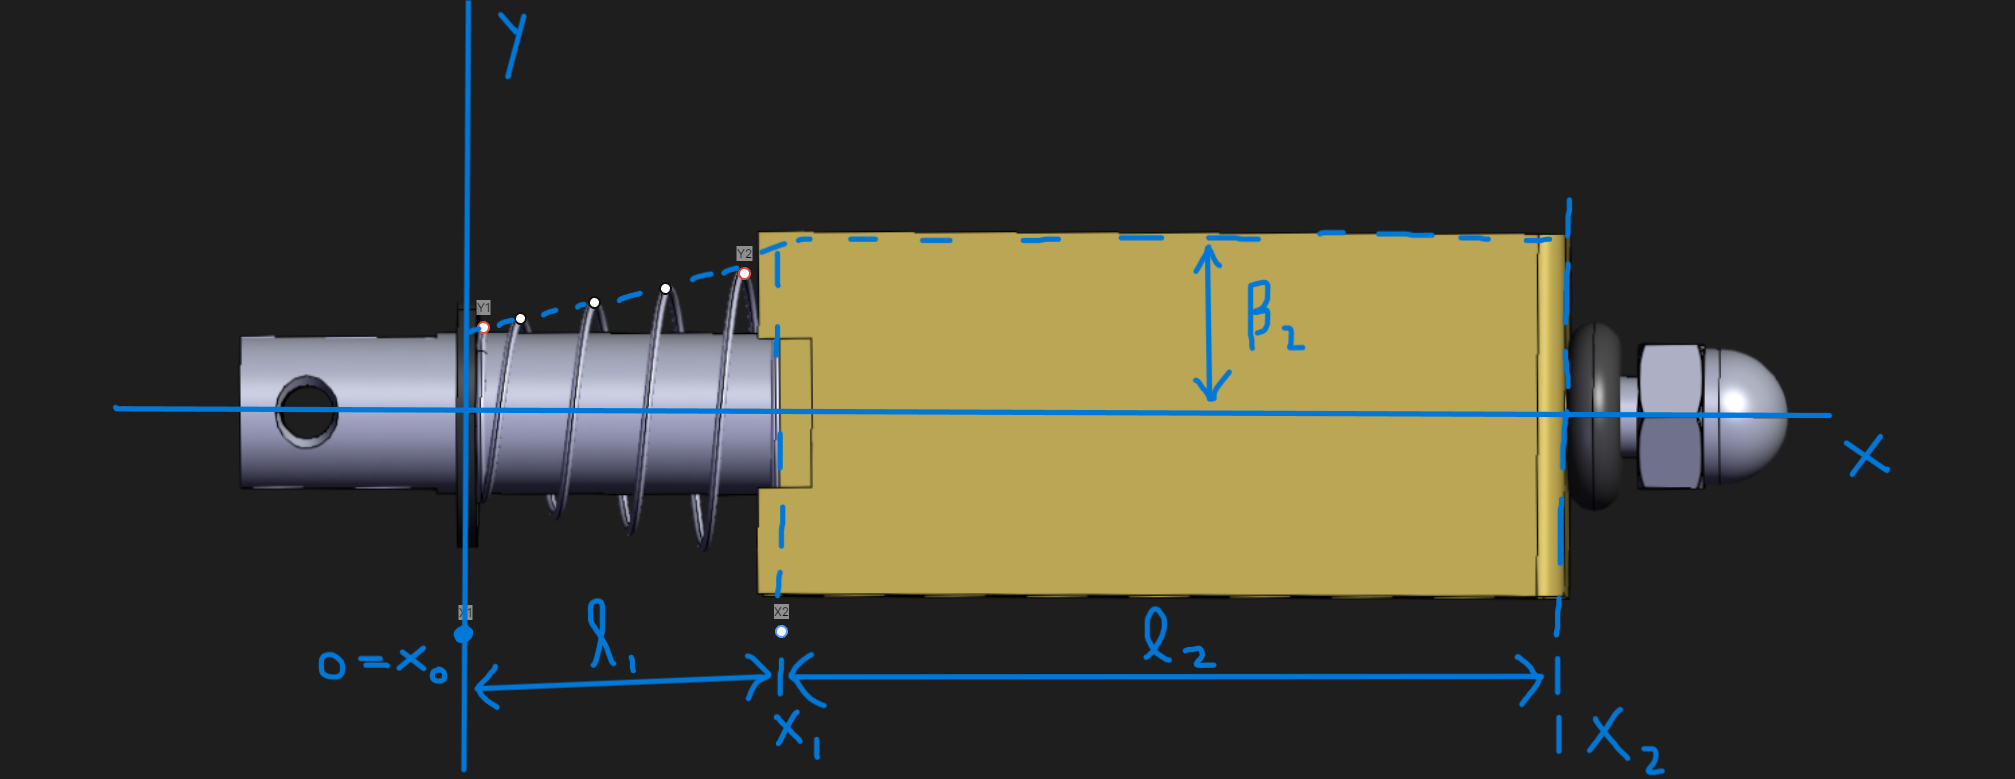
\includegraphics[scale=0.25]{images/solenoidside.png}
    \caption{Solenoid Side View}
    \label{fig:solenoidsideview}
\end{figure}
Using the same point plotter, I found a linear function that modeled the gradient from $x=0$ to $x=x_1$ as a best-fit line -whose \textit{y}-value is the radius as a function of position- over a distance $\ell_1 = 3 cm$ where the radius $\beta(x)$ is increasing. The \textit{y}-intercept of the former half of the piecewise function is the minimum radius, which I measured to be 1cm. The maximum radius, which occurs at $x_1$, is 1.5cm. Moving to the second part of the piecewise function, the radius $\beta_2 = 1.5 cm$ is the constant radius from $x=x_1$ to $x=x_2$ over the length $\ell_2 = 8 cm$.
The piecewise function for radius $\beta(x)$ is
 \begin{equation}
\beta(x) = 
    \begin{cases} 
     0.168001x +0.01, & 0 \leq x < x_1 \\
      0.015, & x_1\leq x\leq x_2
   \end{cases}
\end{equation}
Hence the piecewise function for $A(x)$ is
\begin{equation}
A(x) = 
    \begin{cases} 
     \pi (0.168001x +0.01)^2, & 0 \leq x < x_1 \\
     \pi (0.015)^2, & x_1\leq x\leq x_2
   \end{cases}
\end{equation}
I can substitute $A(x)$ into (\ref{eq:Inductanceeq}), but computing two $L$ values separately, $L_1$ representing the self-inductance of the section on $0 \leq x < x_1$ and $L_2$ for $x_1 \leq x \leq x_2$, each with $\ell_1$ and $\ell_2$ respectively. The number of turns for $L_1$ is $N_1 = 4$, and for $L_2$ it is $N_2 = 10$.
\begin{gather*}
    L = L_1 + L_2 = \int_{0}^{x_1} \mu_0 \frac{N_1^2}{\ell_1^2} A(x) \, dx + \int_{x_1}^{x_2} \mu_0 \frac{N_2^2}{\ell_2^2} A(x) \,dx\\
    = \mu_0  \left( \frac{N_1^2}{\ell_1^2} \int_{0}^{x_1}  \pi (0.168001x +0.01)^2 \, dx + \frac{N_2^2}{\ell_2^2} \int_{x_1}^{x_2}  \pi (0.015)^2 \,dx \right)
    \end{gather*}
Let $u = 0.168001x +0.01$, hence $du = 0.168001 dx $
    \begin{gather}
        \Rightarrow \mu_0 \left( \frac{\pi N_1^2}{0.168001\ell_1^2}\int_{0}^{\frac{x_1}{0.168001}} u^2 \, du + \frac{ N_2^2 \pi (0.015)^2 (x_2 - x_1)}{\ell_2^2}  \right)\\
= \mu_0 \left( \frac{\pi N_1^2}{0.168001\ell_1^2} \frac{(\frac{x_1}{0.168001})^3}{3} + \frac{ N_2^2 \pi (0.015)^2 (x_2 - x_1)}{\ell_2^2}  \right)
    \end{gather}
Substituting for all variables, I get approximately 0.0007940355885 henries for $L$. Hence, the voltage consumed by the inductor is given by
\begin{equation}{\label{eq:voltageinductor}}
    0.0007940355885 \cdot \frac{d^2Q}{dt^2}
\end{equation}
\FloatBarrier
\section{Solving and Applying the Differential Equation}
With my newfound expressions for capacitance, self-inductance, and voltage consumed, I can solve (\ref{eq:differentialequation1}) for the current as a function of time. First, I differentiated with respect to time to make the right-hand side 0, yielding a homogeneous differential equation that I can analytically solve.
\begin{equation}\label{eq:finaldiffeq}
  \frac{d}{dt} \left[ L \frac{di}{dt} + iR+ \frac{1}{C} \int_{0}^{t} i(\tau) \, d\tau \right] =  L \frac{d^2i}{dt^2} + \frac{di}{dt}R+ \frac{1}{C}i = 0
\end{equation}
I know that whatever my final function for $i(t)$ is, it will contain sine and/or cosine term(s) to reflect the alternating current.  I will use $j$ to represent the imaginary unit to avoid confusion with the current. To represent both of these possibilities in a singular form, I assumed that the solution(s) to this equation are in the form 
$$i(t) = e^{zt}, \hspace{10pt} z \in \mathbb{C}$$ 

\noindent Where I am assuming $z$ is some complex number of the form $a \pm bj$. This follows the Euler form, allowing for a representation of alternating current and a solution for the differential equation. Based on this model, I can compute the first and second derivatives of $i$ with respect to time and substitute them into (\ref{eq:finaldiffeq}).
$$ \frac{di}{dt} = ze^{zt} \hspace{3cm} \frac{d^2i}{dt^2} = z^2e^{zt}$$
$$ \therefore 0 = L(z^2e^{zt}) + R(ze^{zt}) + \frac{1}{C} (e^{zt})= (e^{zt}) \left( Lz^2 + Rz + \frac{1}{C} \right) $$
The significance of the constant $z$ is revealed, which are the roots of this new characteristic polynomial, given that $e^{zt}$ can never be zero. Hence, the roots $z_1, z_2$, which should be complex based on the discriminant\footnote{The discriminant is negative for all physically possible dielectric constant values}, are reflected in the solutions to the differential equation:
\begin{equation}
    i_1(t) = e^{z_1 t} \hspace{3cm} i_2(t) = e^{z_2 t}
\end{equation}
\noindent The complete solution can then be written as 
$$ i(t) = A_1i_1(t) + A_2i_2(t) $$
Where $A_1$ and $A_2$ are arbitrary constants whose physical significance can be determined later - for now, they are just amplitude. This result arises from the \textbf{Principle of Superposition} - both currents exist simultaneously as functions of time, so the effective current function can be determined by adding the two solutions to the differential equation. Using my derived values for $L, R, C$, I can find the roots of this polynomial and hence my current as a function of time and $\kappa$.
\begin{equation}
    z_{1,2} = -16.634086492588956 \pm 
\sqrt{276.6928334429304 - \frac{8.96446366 \times 10^{14}}{\kappa}}
\end{equation}
To simplify this, I will write the roots in terms of $a$ and $bj$, where $a=276.6928334429304$ and $bj$ is the complex-valued root. $b$ is then equal to the root divided by $j$. The first solution for current as a function of time and $\kappa$ is\footnote{All trigonometric terms have the same input as I used the complex-conjugate identity for Euler's method, yielding $e^{-j\theta} = \cos(\theta) - j\sin(\theta)$}:

\begin{gather*}
    \textbf{Re}(i(t, \kappa)) = A_1e^{z_1 t} + A_2e^{z_2 t} \\
    \therefore e^{z_1 t} + e^{z_2 t} =  e^{-at}\left(e^{b{t}} + e^{-bt}\right)\\
   = e^{-at} \left( \cos(bt) + j\sin(bt) + \cos( bt) - j\sin( bt) \right)\\
    = 2e^{-at} \cos(bt)
\end{gather*}
This is the real solution, and to eliminate the extraneous 2, I let $A_1 = A_2 = \frac{1}{2}$ in this case. Note that I assumed that the square root would yield a complex number (based on the range of $\kappa$ I found online), so the $j$ in the denominator ensures continuity with Euler's form, only including the coefficient. Meanwhile, for the second solution, which is imaginary, I take the difference between the exponentials, using a similar method:
\begin{gather*}
    j \cdot \textbf{Im}(i(t, \kappa)) = A_1e^{z_1 t} - A_2e^{z_2 t} \\
    \therefore e^{z_1 t} - e^{z_2 t} = 2j e^{-at} \sin(bt)
\end{gather*}
The second solution is still imaginary after simplification, so I decided to let $A_1 = \frac{1}{2j} $ and $A_2 = -\frac{1}{2j}$ in this case, which removes the $2j$ term at the front. Hence,
\begin{gather*}
    i(t,\kappa) =   \textbf{Re}(i(t, \kappa)) + j \cdot \textbf{Im}(i(t, \kappa))\\
    =   e^{-at} \left( A_1\cos(bt) + A_2\sin(bt) \right) \\ 
   = \left. A_3 e^{-at} \cos(bt - \phi(\kappa)) \right\vert \, (b, t,\kappa) \in \mathbb{R}
\end{gather*}
Where $A_3$ is a new amplitude equivalent to $\sqrt{A_1 ^2 + A_2 ^2}$ and $\phi$ is the phase shift \footfullcite{pauls_notes_complex_roots}.

\section{Tuning}
From this function, the angular frequency $\omega = b $. Hence, for the audio frequency ranges given below, I can now compute the optimal dielectric material for the various circuits, using the relation $\omega = 2\pi f_{\text{avg}}$, where $f$ is the range of audio frequencies. I will use the average of each range to calculate $\omega_{\text{0}}$ and consequently $\kappa$. I will then choose a candidate for the dielectric constant by requiring its $\kappa$ to be within $50\%$ of the ideal one, as there is a lenient range for the frequencies. I collected data on the dielectric constants of various materials in \textbf{Table 6}. Based on my tuning presets, I will compute $A_3$ for my preferences. I have +20\% decibels for some frequency ranges, and for others, -10\% decibels, labeled EQ. Assuming a baseline volume of 1 decibel, I will write $A_3$ as the increase or decrease from that baseline, with a 20\% increase being $A_3 = 1.2$, for example. To calculate the phase shift for each circuit, I must use the impedance $Z$ of the circuit\footfullcite{CeramTec2023Dielectric}. Impedance is a measure of the opposition to alternating current within a circuit, decreasing electric flow and, consequently, the volume of audio generated. The impedance has both real and imaginary parts, and is given by\footfullcite{Impedance}:
\begin{equation}
    Z = R + j\left(\omega L -\frac{1}{\omega C}        \right)
\end{equation}
\noindent The phase shift is equal to $\textbf{arg}(Z)$, hence
\begin{gather*}
    \phi(\kappa) = \arctan(\frac{\textbf{Im}(Z)}{\textbf{Re}(Z)} ) = \arctan(\frac{\omega L -\frac{1}{\omega C}}{R})
\end{gather*}
I used this formula to calculate $\phi$ for each frequency range\footfullcite{PhaseShift}.

\begin{table}[h!]
    \centering
    \begin{tabular}{c|c|c|c|c|c|c}
      $f$ (kHz)  & $\omega_{\text{0}}$ (rad/s)& $\kappa$ & Dielectric & $\phi $ (rad) &EQ (\% db) & $A_3$\\ \hline
       0-16  & 50,265.44 & 354800.769& N/A & $-16.52 \times 10^{-5}$ & 5.0 & 1.05 \\
       16-32  &150,796.32  & 39422.312& N/A& $-5.423\times10^{-5}$& 15 & 1.15 \\
       32-48  & 251,327.20 & 14192.032& \ce{CaCu_3 Ti_4 O_12}& $-3.156\times 10^{-5}$&-10. & 0.90 \\
       48-64  & 351,858.08  & 7240.833& \ce{CaCu_3 Ti_4 O_12}& $ -2.149 \times 10^{-5}$&-20. & 0.80\\
       64-80 & 452,388.96  & 4380.257& \ce{BaTi(K_3 5OOH)} & $ -1.562 \times 10^{-5}$& 40. & 1.4\\
       80-96  & 552,919.84 & 2932.238& \ce{SrTiO_3}& $ -1.166 \times 10^{-5} $& -30.  & 0.70 \\
    \end{tabular}
    \caption{Different Quantities of the Current Function for Audio Frequencies}
    \label{tab:audiotuningtable}
\end{table}
\FloatBarrier
\noindent 
\noindent Finally, the following current functions of $t$ were found with each dielectric candidate's $\kappa$ used to find the angular frequencies -excluding the first two frequency bands $f_{1,2}$- to create the 6 signal circuits, following the same descending order as the table\footfullcite{DielectricConstants}. These first two bands use the ideal angular frequencies, as no dielectrics exist within a $50\%$ range of their $\kappa$:
\begin{gather*}
f_1: i(t) = 1.05 \, e^{-16.6 \, t} \cos\left(50200 \, t + 16.5 \times 10^{-5} \right) \\
f_2:i(t) = 1.15 \, e^{-16.6 \, t} \cos\left(151000 \, t + 5.42 \times 10^{-5} \right) \\
f_3:i(t) = 0.90 \, e^{-16.6 \, t} \cos\left(299000 \, t + 3.16 \times 10^{-5}\right)\\
f_4:i(t) = 0.80 \, e^{-16.6 \, t} \cos\left(299000 \, t + 2.15 \times 10^{-5}\right) \\
f_5:i(t) = 1.40 \, e^{-16.6 \, t} \cos\left(726000 \, t + 1.56 \times 10^{-5}\right)\\
f_6:i(t) = 0.70 \, e^{-16.6 \, t} \cos\left(669000 \, t + 1.17 \times 10^{-5}\right)
\end{gather*}

\section{Conclusion}
\noindent My approach to inducing phase changes through the dielectric constant resulted from an inability to alter the circuit in any other manner, as I did not have the equipment to change the separation distance between capacitor plates, which would have been simpler and allowed me to create physically possible currents for the 2 lowest frequencies: $f_1$ and $f_2$. Generally, the required dielectric constants were extremely high, so decreasing the plate separation ($\kappa \propto
d$) would make tuning possible for me to carry out in reality - many of the required dielectric candidates are not accessible to the general population. This would greatly simplify calculations and allow for future steps with more circuits, perhaps 8 or 12 frequency intervals for more precise frequency coverage.\\
\noindent I learned to apply physical intuition to mathematics, particularly when solving (\ref{eq:finaldiffeq}). The initial conditions -in this case, boundary conditions- I am usually given for differential equations had to be physically derived through examinations of important points like \textit{y}-intercepts. Furthermore, using physical observations to justify assumptions for the structure of solutions was a new way of approaching math that I had not experienced beforehand. While the calculation of the constants was somewhat approximate, I was able to minimize them by noting physical measurements and finding methods that best leveraged specific domains and constants toward precision, such as using a Maclaurin Series for a tiny domain of integration and Euler's method for a larger one.
\noindent In addition, the evaluation of my constants yielded an unintended but desirable band-filter property of my circuit, which is dependent on impedance. At a certain angular frequency $\omega_0$, the inductive ($\omega L$) and capacitive ($\frac{1}{\omega C}$) reactances cancel out, resulting in the circuit having minimum impedance and maximum current-flow.
\begin{equation}
    Z(\omega_0) = R + j\left(\omega_0 L -\frac{1}{\omega_0 C} \right) = 0
\end{equation}
This $\omega_0$ corresponds to the resonant frequency $f_0 = \frac{\omega_0}{2\pi}$. As $\omega \rightarrow \omega_0$, the impedance decreases and $A_3$ increases, while a further deviation from the resonant frequency results in higher impedance and lower volume. This is an important aspect of noise isolation, allowing for targeted frequencies to stand out, but it can only be properly utilized with over 16 signal circuits. For example, a song with strong, feminine vocals can sound extremely clear, but without enough signal circuits, some frequencies will become absent without a nearby ``$f_0$ pole'', and it will feel somewhat incomplete.
\newpage
\section{Appendix}
\begin{table}[h!]
\centering
\begin{tabular}{|c|c|}
\hline
\textit{x} & \textit{y} \\ \hline
0.03289473684210526 & 0.013928571428571429 \\
0.05921052631578947 & 0.02142857142857143 \\
0.08947368421052632 & 0.02892857142857143 \\
0.11578947368421053 & 0.03642857142857143 \\
0.15263157894736842 & 0.04285714285714286 \\
0.18421052631578946 & 0.03750000000000000 \\
0.21052631578947367 & 0.03214285714285715 \\
0.24473684210526314 & 0.024642857142857143 \\
0.2723684210526316 & 0.018214285714285714 \\
0.30526315789473685 & 0.010714285714285714 \\
0.017105263157894738 & 0.007500000000000001 \\
0.13421052631578947 & 0.04071428571428572 \\
0.16842105263157894 & 0.04178571428571429 \\
0.3447368421052632 & 0.0010714285714285715 \\
0.38026315789473686 & -0.007500000000000001 \\ \hline
\end{tabular}
\caption{\textit{x} and \textit{y} Data Points for Best Fit Line}
\label{table:xydata}
\end{table}

\begin{table}[h!]
    \centering
\begin{longtable}{cc}
\hline
Composition & Dielectric constant \\
\hline
\endfirsthead

\hline
Composition & Dielectric constant \\
\hline
\endhead

\hline
\endfoot

\hline
\endlastfoot

\ce{SiO_2} & 3.9 \\
\ce{Al_2O_3} & 9  \\
\ce{ZrO_2} & 29  \\
\ce{HfO_2} & 25 \\
\ce{La_2O_3} & 30  \\
\ce{LaAlO_3} & 30  \\
\ce{Nb_2O_5} & 35  \\
\ce{TiO_2} & 95  \\
\ce{BaTiO_3} & 1700 \\
\ce{SrTiO_3} & 2000 \\
\ce{BaTi(K_3 5OOH)} & 4500 \\
\ce{CaCu_3 Ti_4 O_{12}} & 10000 \\
\end{longtable}
   \caption{Dielectric Constants of Various Materials} 
    \label{dielectricconstants}
\end{table}
\printbibliography
\end{document}


